\section{Proposed Method}
Existing specification-based malware detectors can be utilized if we extract
the correlation between shadow processes efficiently, because with that correlation
we are able to reconstruct the original system call graph from system call sequences
of shadow processes. In this section, we propose the design of a system method to extract the correlation.

\subsection{Problem Scope}
We focus on only shadow attacks that performs Inter-Process Communication, or IPC, via unix domain socket.

\cite{Weiqin:ShadowAttack} showed prototype implementation of a compiler
that takes existing malware as input and outputs the executable of malware of shadow-attack version.
Therefore, it is reasonable to infer that shadow attacks based on IPC through unix domain socket
are highly feasible, and they should be considered as a significant threat.

\subsection{Key Concepts (tentative)}
As mentioned before, shadow attacks are the strategy where malware exports its critical system calls
to shadow processes and hyde its malicious behavior.
\cite{Weiqin:ShadowAttack} listed examples of system calls that are critical for malware's intent,
shown in \Tref{tab:critical-system-calls}.

\begin{table*}[t]
  \caption{Examples of critical system calls. This table is reconstructed from \cite{Weiqin:ShadowAttack} by the author from.}
  \centering
  \begin{tabular}{|l|l|}
    \hline
    \textbf{Function Category} & \textbf{System Call}                     \\
    \hline
    File I/O operation         & open, read, write                        \\
    \hline
    Network                    & socket, connect, recv, send, read, write \\
    \hline
    Process management         & exec, execl                              \\
    \hline
  \end{tabular}
  \label{tab:critical-system-calls}
\end{table*}

Among these system calls, file-related and network-related system calls handle file descriptors:
\texttt{open} and \texttt{socket} create a new file descriptor,
while others access the file tied to the file descriptor or perform network communication.
So shadow processes need to transfer file descriptors to each other to perform the file-related and
network-related system calls. This concept is shown in \Fref{img:fd-transfer}.
To our best knowledge, file descriptor transfer through unix domain socket is a technology that, although not uncommon
in cloud-native environments \cite{Envoypro3:online,HAProxyT74:online},
is relatively rare in traditional Linux server environments
(that would be because the technology introduces unnecessary complexity and overhead in the system).
This situation makes the file descriptor transfer a unique characteristic of shadow attacks.

\begin{figure*}[t]
  \begin{center}
    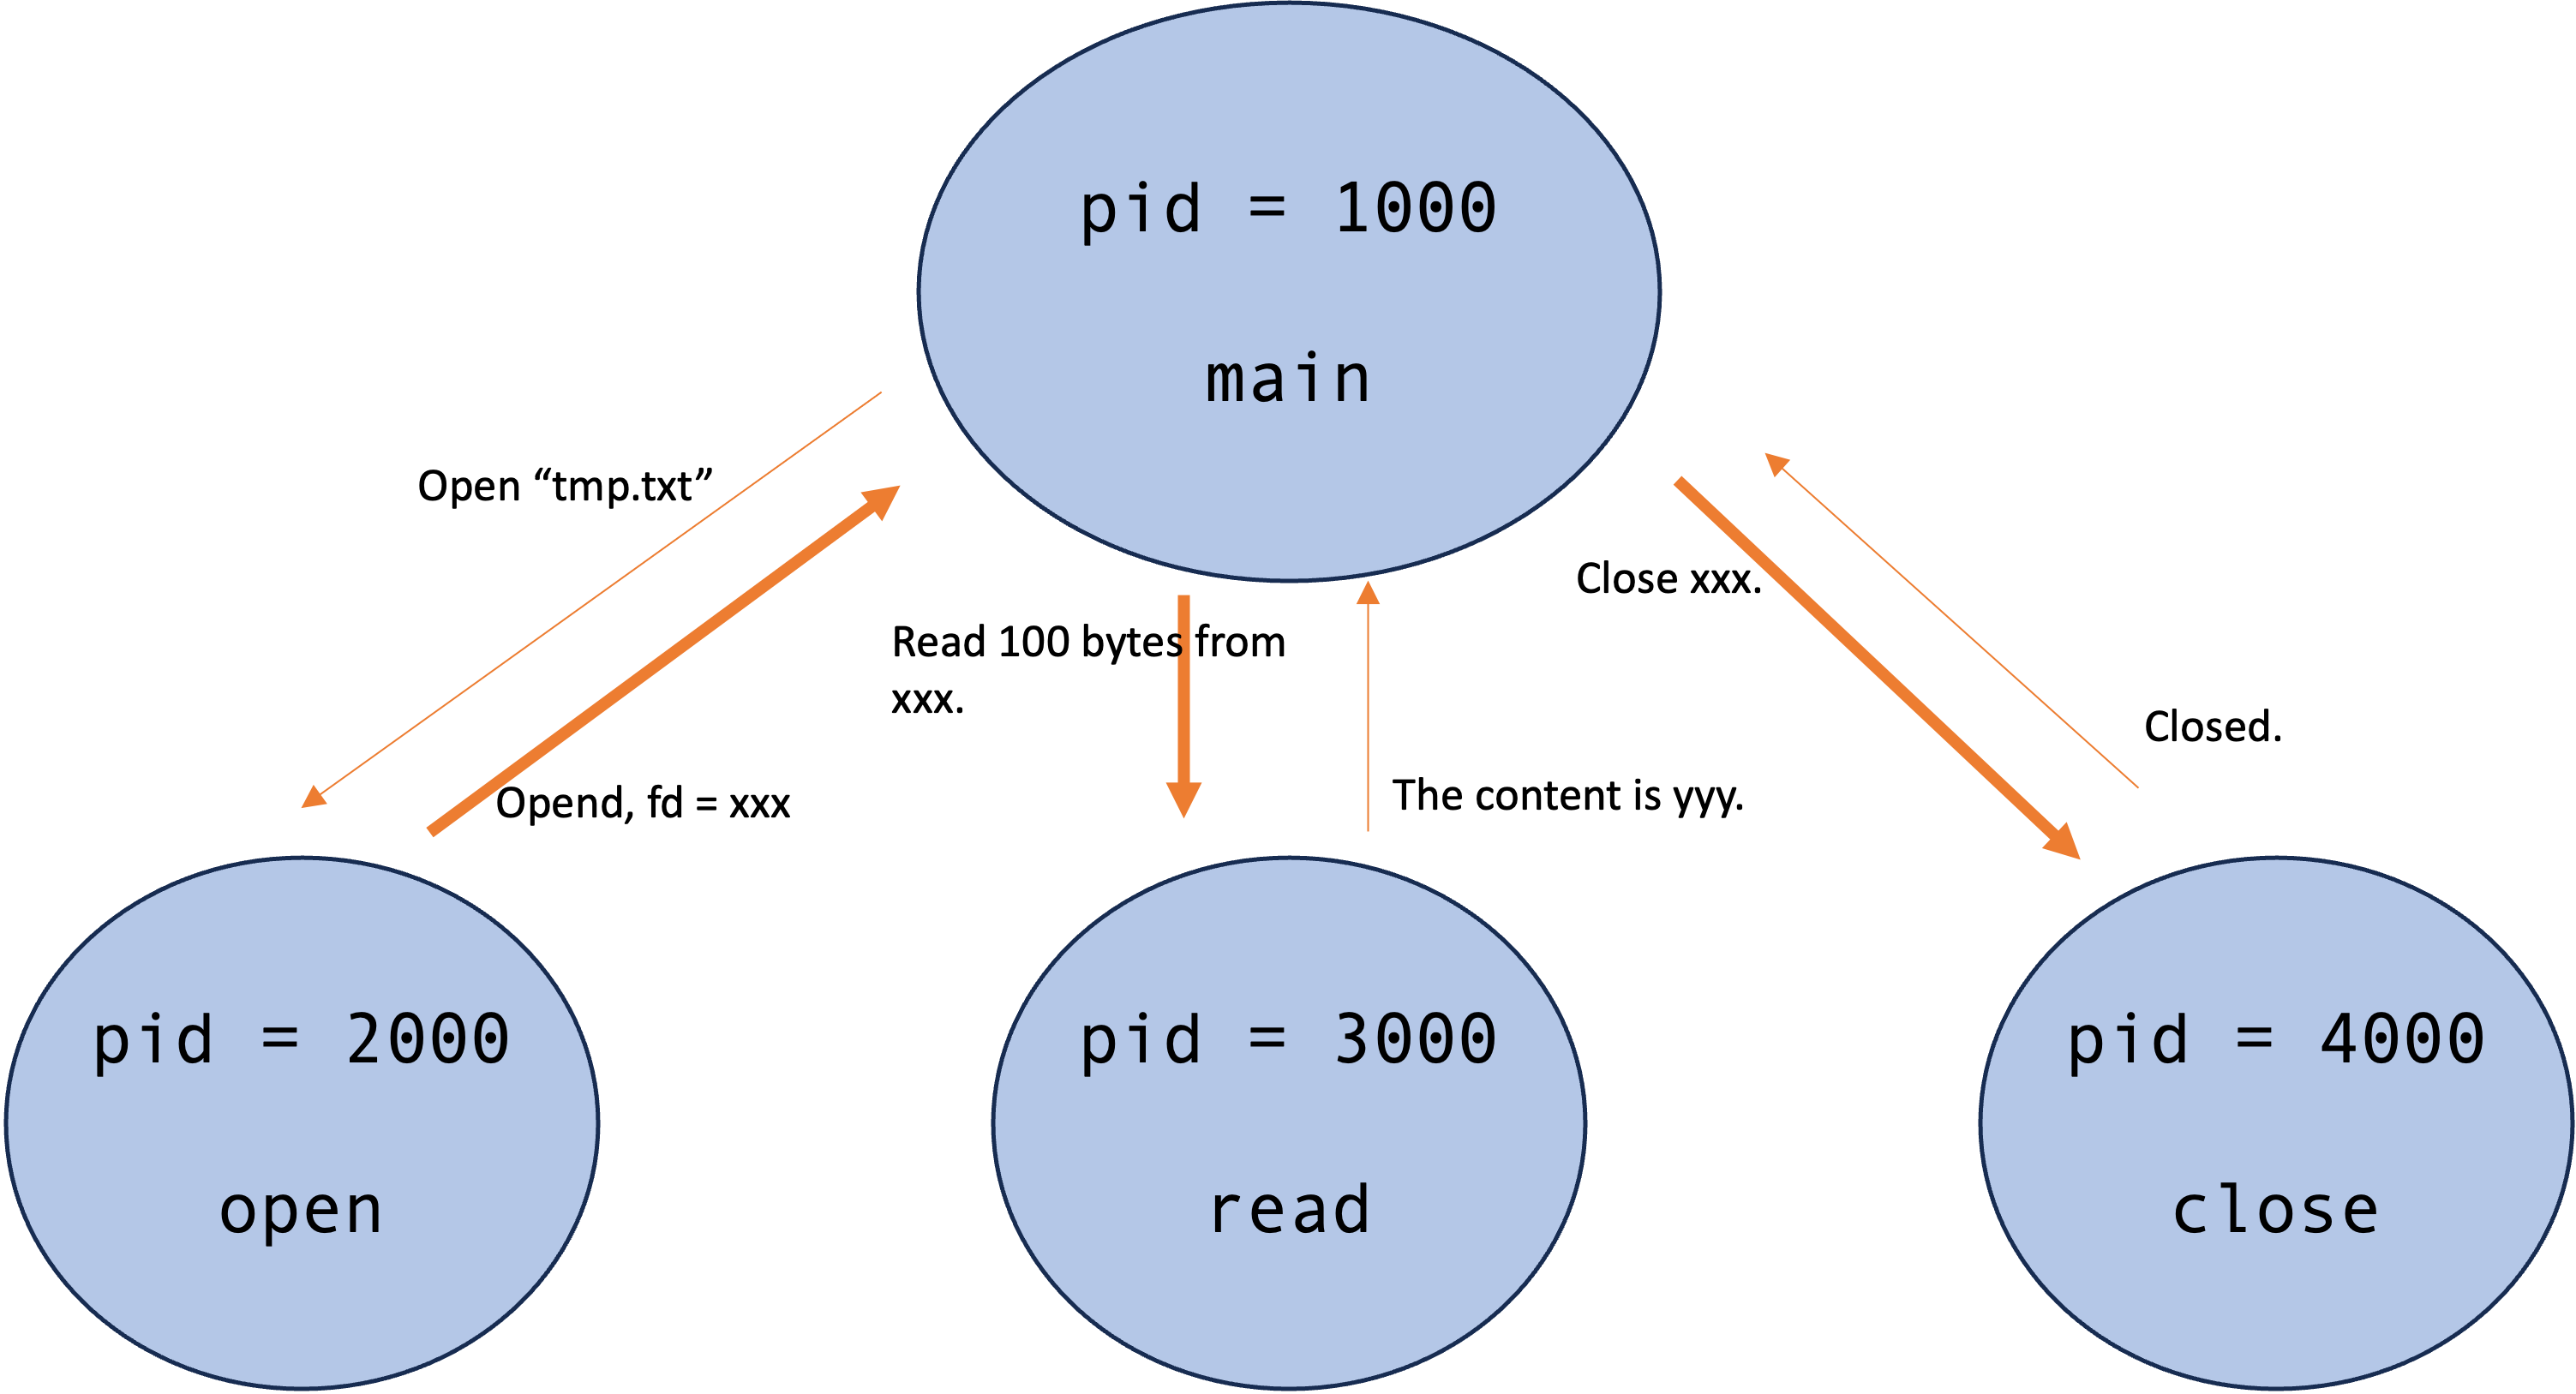
\includegraphics[width=1.8\columnwidth]{./img/fd_transfer.png}
  \end{center}
  \caption{Illustration of the concept of file descriptor transfer between shadow processes.
    The main process requests the shadow process to execute system calls, along with the required arguments.
    The thick arrows indicate the transfer of file descriptors over the control messages exchanged through IPC.}
  \label{img:fd-transfer}
\end{figure*}

\subsection{Design Overview}
The overview of proposed method is shown in \Fref{img:proposal-overview}.
Our system consists of the three components: the eBPF program, the eBPF map, and the user space program.
Each of them are described in detail in the following subsections.
\begin{figure*}[t]
  \centering
  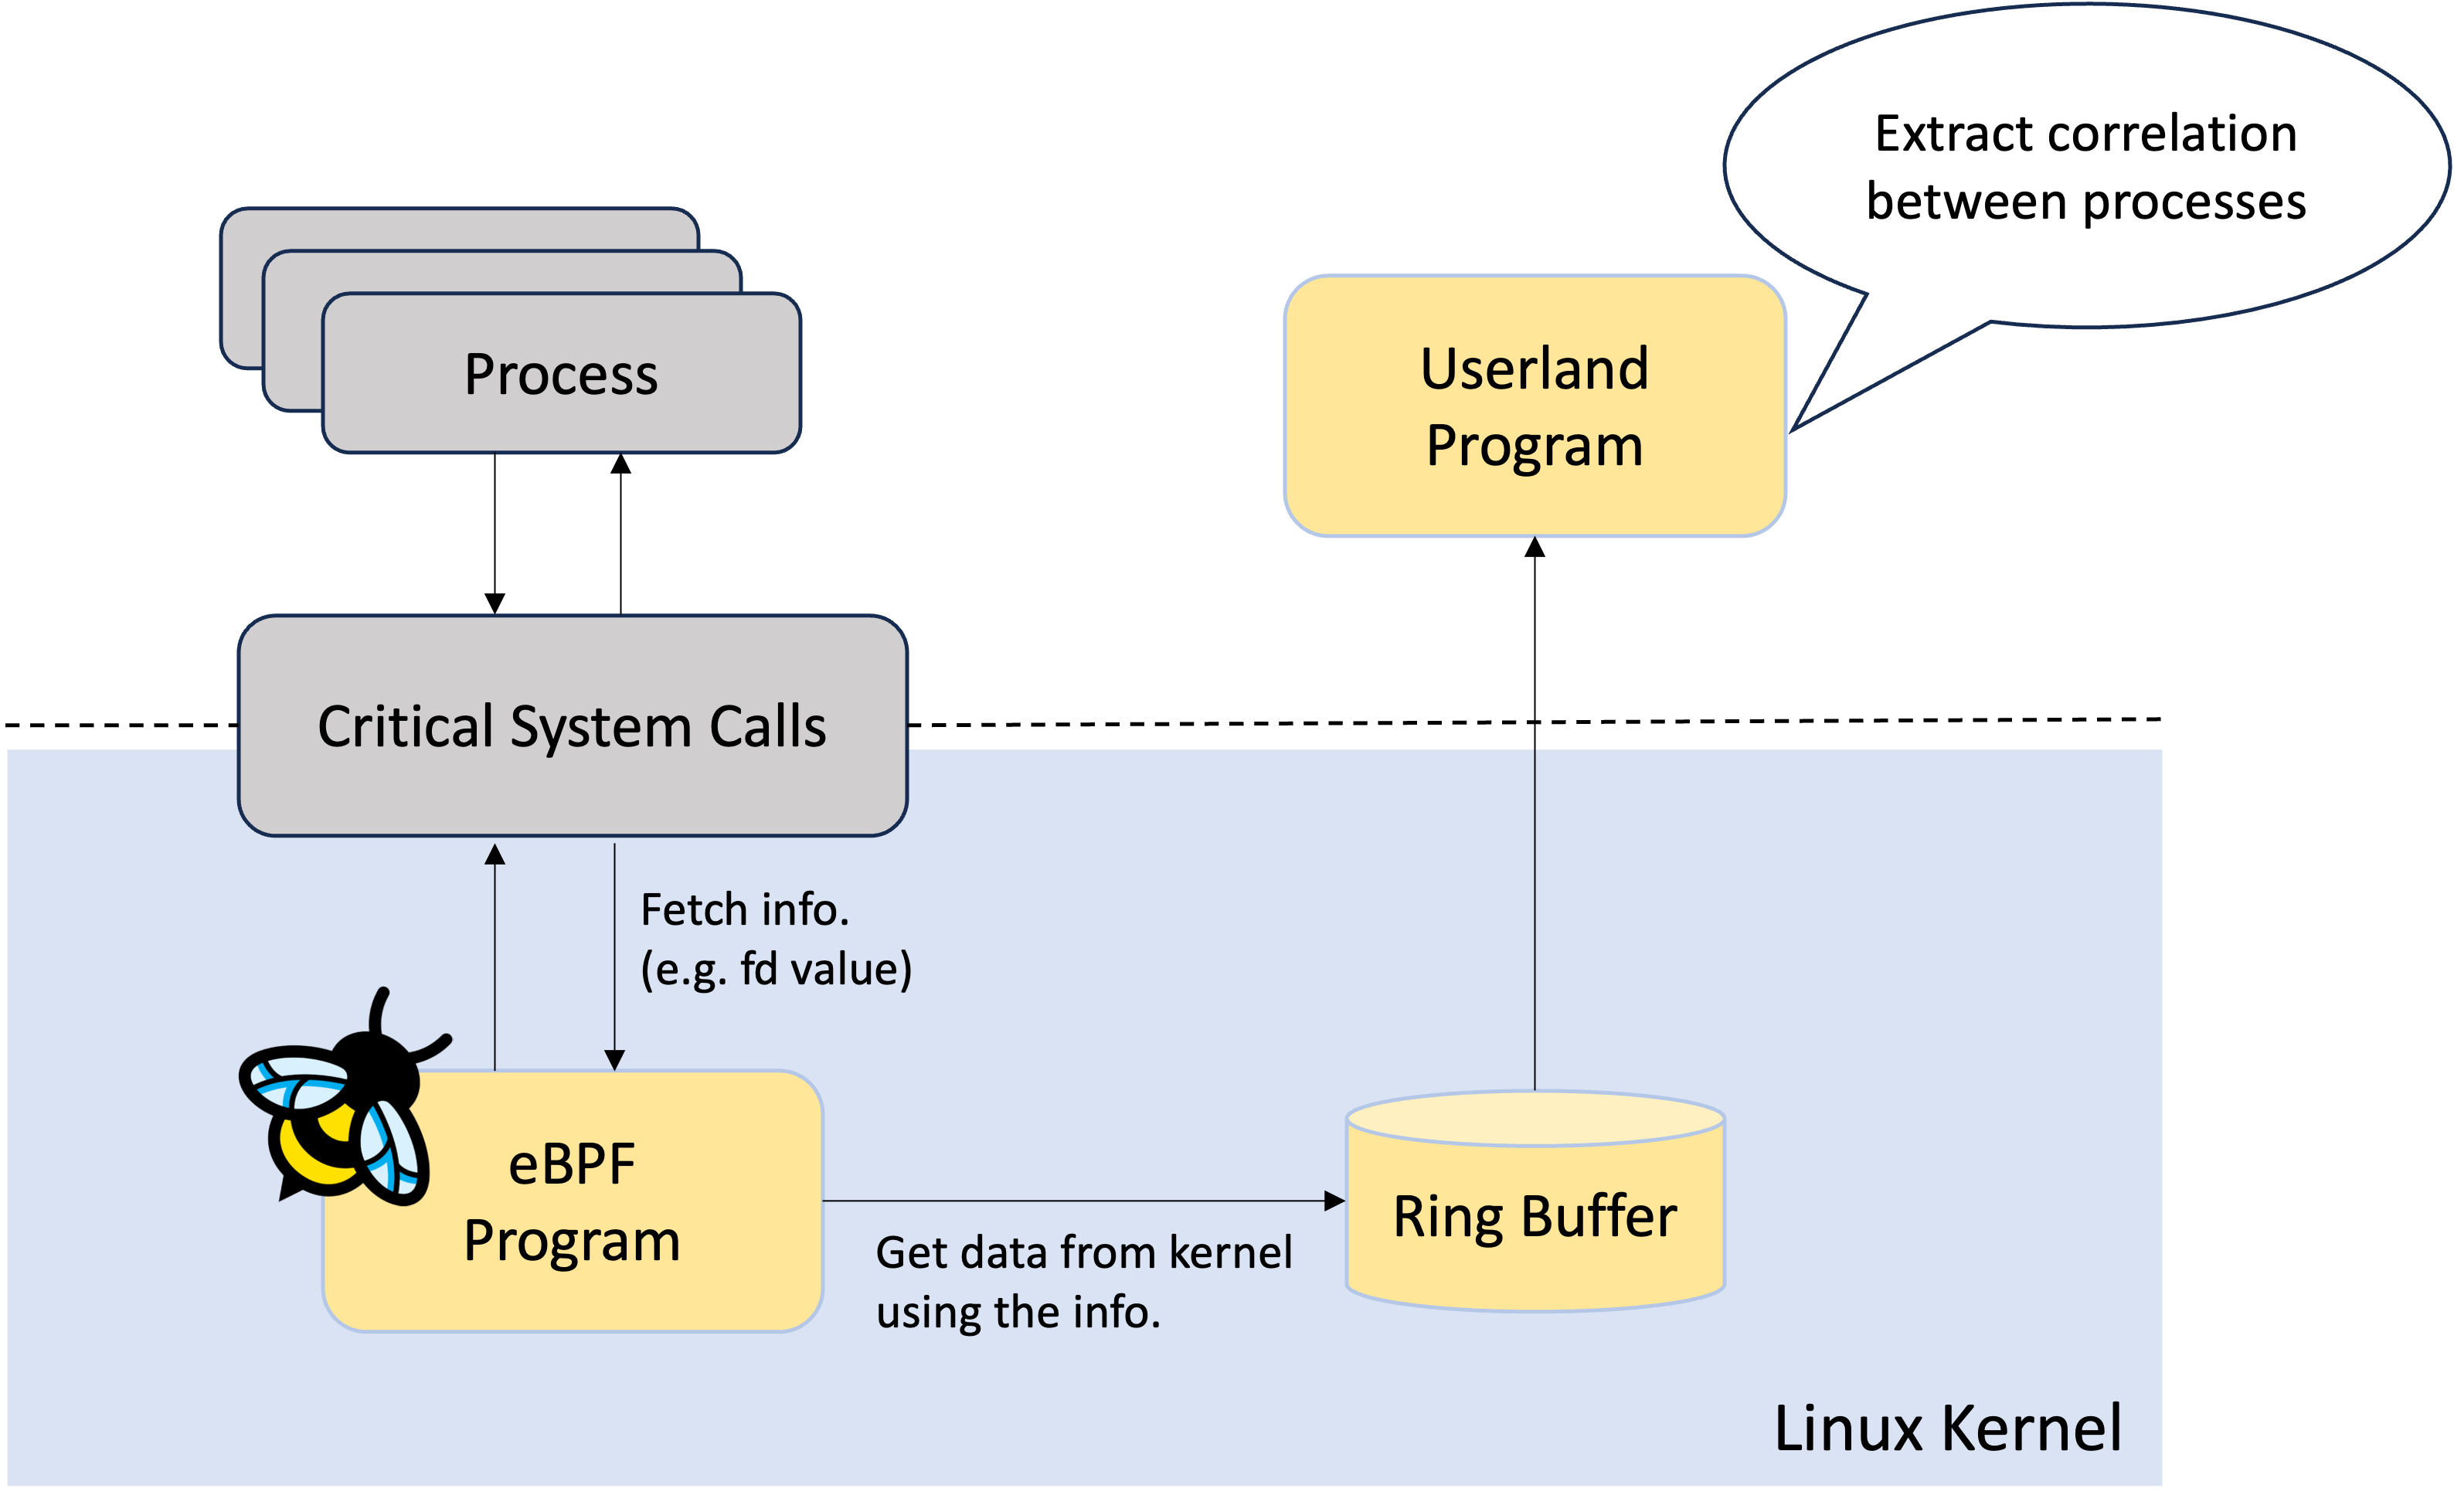
\includegraphics[width=1.5\columnwidth]{./img/proposal_overview.png}
  \caption{Overview of the proposed method. Our research is not
    affiliated with or otherwise sponsored by eBPF Foundation\cite{BrandGui21:online}.}
  \label{img:proposal-overview}
\end{figure*}

\subsubsection{Details of eBPF Program}
We use fentry/fexit \cite{learning-ebpf}, eBPF features that were introduced in kernel version 5.5,
to efficiently attach the eBPF program to the entry of exit point of specific system calls.

In this system the eBPF program is attached to the file-related system calls such as \texttt{open} or \texttt{read},
and gets the value of file descriptor passed to the system call as an argument.
It retrieves the pointer of \texttt{task\_struct} \cite{schedhin43:online} of the process that issued the system call,
and dereferences it to read the file descriptor array in a way that meets the demand of eBPF verifier.
Using this array,
it reads the pointer to the open file object (named \texttt{struct file} \cite{fshinclu57:online} internally)
corresponding to the specified file descriptor.

Then the program populates the eBPF map with the entry of data structure that
contains pid (process id), ppid (parent pid),  an integer that indicates which system call was issued,
and the pointer value to the file structure.

\subsubsection{Details of eBPF Map: Ring Buffer}
eBPF map is a data structure that allows data sharing between user space and kernel space, and
we select ring buffer as the type of eBPF map for this system because read from user space
and write from kernel space happen at the same rate.

As described in the previous subsection, the eBPF program populates the ring buffer
every time the file-related system call is issued.

\subsubsection{Details of User Space Program}
\textbf{It needs to be noticed that some implementation details remain to be finalized, which could
  lead to further refinements in the future.
}

The user space program stores which process accesses a specific open file object (or \texttt{struct file})
as a key-value pair in a hash table, and infers that there is a correlation between the processes
A and B if both of them access the same object.
% finds he correlation between shadow processes by inspecting
% data of open file objects in kernel memory that are associated with opened files.
The \texttt{task\_structs} of different processes have open file objects separately
even if they are opening the same file.
However, when the file objects are shared between the processes explicitly via unix domain socket, or
when they are in parent-child relationship, the open file objects are shared.
Since the program knows whether given two processes are in parent-child relationship or not
by checking pid and ppid,
it can infer that the processes are transferring file descriptors through unix domain socket,
and thus they are shadow processes
if they access the same open file object and they are independent processes.

% \begin{algorithm}
%   \caption{foooooooo}
%   \label{algo:1}
%   \begin{algorithmic}[1]
%     \Procedure{Insertion-Sort}{$A$}
%     \State{$h = hash\_table$}
%     \While{Read $entry$ from ring buffer}
%     \State{${file\_obj} = entry.obj$}
%     \If{$file\_obj$ is not in $h$}
%     \State{Insert $file\_obj$ to $h$}
%     \State{Continue}
%     \EndIf

%     \If{$entry.pid$ is not in $h[file\_obj]$}


%     \State{$i = j - 1$}
%     \State{$A[i + 1] = k$}
%     \EndWhile
%     \EndProcedure
%   \end{algorithmic}
% \end{algorithm}
